\documentclass[twocolumn, amsmath, amsfonts, amssymb, trackchanges]{aastex62}
\usepackage{mathtools}
\usepackage{natbib}
\usepackage{bm}
\newcommand{\vdag}{(v)^\dagger}
\newcommand\aastex{AAS\TeX}
\newcommand\latex{La\TeX}


\newcommand{\Div}[1]{\ensuremath{\nabla\cdot\left( #1\right)}}
\newcommand{\DivU}{\ensuremath{\nabla\cdot\bm{u}}}
\newcommand{\angles}[1]{\ensuremath{\left\langle #1 \right\rangle}}
\newcommand{\td}[1]{\ensuremath{\widetilde{#1}}}
\newcommand{\KSstat}[1]{\ensuremath{\overline{\text{KS}(#1)}}}
\newcommand{\grad}{\ensuremath{\nabla}}
\newcommand{\RB}{Rayleigh-B\'{e}nard }
\newcommand{\stressT}{\ensuremath{\bm{\bar{\bar{\Pi}}}}}
\newcommand{\lilstressT}{\ensuremath{\bm{\bar{\bar{\sigma}}}}}
\newcommand{\nrho}{\ensuremath{n_{\rho}}}
\newcommand{\approptoinn}[2]{\mathrel{\vcenter{
	\offinterlineskip\halign{\hfil$##$\cr
	#1\propto\cr\noalign{\kern2pt}#1\sim\cr\noalign{\kern-2pt}}}}}

\newcommand{\appropto}{\mathpalette\approptoinn\relax}
\newcommand{\pro}{\ensuremath{\text{Ro}_{\text{p}}}}
\newcommand{\con}{\ensuremath{\text{Ro}_{\text{c}}}}

\usepackage{color}
\newcommand{\gv}[1]{{\color{blue} #1}}

%% Tells LaTeX to search for image files in the 
%% current directory as well as in the figures/ folder.
\graphicspath{{./}{figs/}{../tex/figs/}}


\received{\today}
\revised{??}
\accepted{??}%\today}
\submitjournal{ApJ}

%%%%%%%%%%%%%%%%%%%%%%%%%%%%%%%%%%%%%%%%%%%%%%%%%%%%%%%%%%%%%%%%%%%%%%%%%%%%%%%
%% TITLE & AUTHORS
\shorttitle{Stratified Thermals}
\shortauthors{Anders et al.}


\defcitealias{lecoanet&jeevanjee2018}{LJ19}
\newcommand{\LJ}{\citetalias{lecoanet&jeevanjee2018}}

\begin{document}
\title{Entrainment of low Mach number thermals in stratified domains}

\correspondingauthor{Evan H. Anders}
\email{evan.anders@colorado.edu}

\author[0000-0002-3433-4733]{Evan H. Anders}
\affil{Dept. Astrophysical \& Planetary Sciences, University of Colorado -- Boulder, Boulder, CO 80309, USA}
\affil{Laboratory for Atmospheric and Space Physics, Boulder, CO 80303, USA}
\author[0000-0002-7635-9728]{Daniel Lecoanet}
\affil{Princeton Center for Theoretical Science, Princeton, NJ 08544, USA}
\affil{Department of Astrophysical Sciences, Princeton, NJ 08544, USA}
\author[0000-0001-8935-219X]{Benjamin P. Brown}
\affil{Dept. Astrophysical \& Planetary Sciences, University of Colorado -- Boulder, Boulder, CO 80309, USA}
\affil{Laboratory for Atmospheric and Space Physics, Boulder, CO 80303, USA}


\begin{abstract}
``Entropy rain,'' or the downard propagation of low entropy fluid, has been hypothesized as a dominant mechanism for carrying the solar luminosity in light of the recent Solar Convective Conundrum.
One possible dynamical manifestation of these ``raindrops'' is that of dense, propagating vortex rings, referred to as ``thermals'' in the context of Earth's atmosphere.
In this work, we develop an analytical theory describing entrainment in dense, antibuoyant vortex rings in stratified atmospheres.
We show that this theory describes the evolution of laminar, axisymmetric thermals in highly stratified atmospheres and into the boussinesq limit.
We discuss what the evolution of these thermals implies for the entropy rain hypothesis.
\end{abstract}

\keywords{hydrodynamics --- turbulence --- entrainment}

%%%%% Body of the paper
%%%%%%%%%%%%%%%%%%%%%%%%%%%%%%%%%%%%%%%%%%%%%%%%%%%%%%%%%%%%%%%%%%%%%
%% INTRODUCTION
\section{Introduction}
\label{sec:intro}
Recent observations of solar convection have revealed a convective conundrum.
Power spectra of horizontal velocities show weaker flows than anticipated at large length scales \citep{hanasoge&all2012, greer&all2015}.
These obserations cast doubt on the existence of ``giant cells'' driven by deep convection which should manifest as powerful, large-scale motions at the solar surface and throughout the solar convection zone. 
This discrepancy between theory and observations has called into question our fundamental understanding of convection, sparking numerous targeted investigations the nature of convection in the Sun  \citep{featherstone&hindman2016, omara&all2016, cossette&rast2016, kapyla&all2017, hotta2017}.

\cite{spruit1997} hypothesized that convective motions in the Sun may be driven entirely by cooling at the solar surface, and \citet{brandenburg2016} expanded upon this ``entropy rain'' hypothesis. 
Brandenburg's work includes a careful expansion of mixing length theory to incorporate flux contributions from nonlocal convective motions, and handles this theory in a horizontally-averaged sense.
He includes some discussion of possible flow morphologies which could be manifestations of this entropy rain, and even includes some brief simulations of propagating Hill vortices. 
However, these simulations and discussions did not include include a fundamental piece of entropy rain: its entropic signature deviates from the background atmosphere.
Entropy rain is dense, and the effects of antibuoyant forces will modify its dynamics.

If entropy rain does evolve into downward propagating, dense vortex rings, it is important to understand how the filling factor of these basic convective elements is affected by their entropy signature. 
In the context of Earth's atmosphere, ``thermals,'' or buoyant fluid regions which evolve into rising vortex rings, are thought to be the nucleus of cloud formation. 
Atmospheric cloud-forming thermals always rise, but the term is also used for the reverse, falling process.
The evolution of thermals in the Boussinesq limit has been well studied in the laboratory for decades \citep[see e.g.][]{morton&all1956, scorer1957}, and more recently have been studied through Direct Numerical Simulation (DNS) in the laminar and turbulent regime \citep{lecoanet&jeevanjee2018}. 
One fundamental result of these studies of thermals is that they experience a large degree of entrainment characterized by radial expansion and decceleration of propagation velocity.
However, we do not know of a study in which the propagation of these thermals, and thus the nature of their entrainment, is affected by a significant atmospheric stratification.

\begin{figure}[t!]
    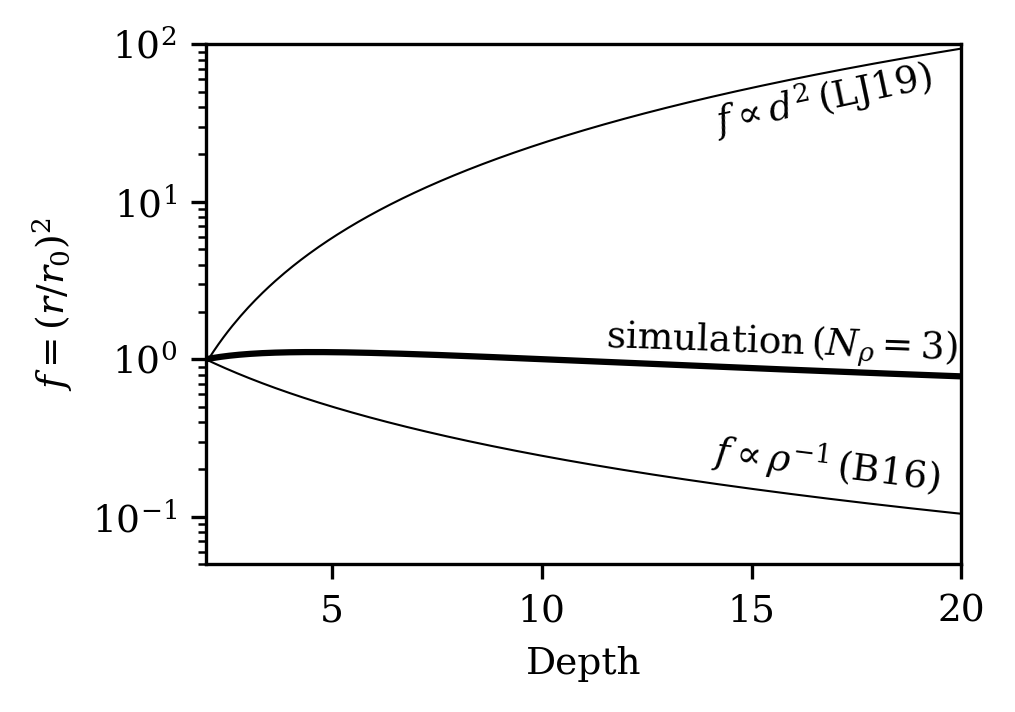
\includegraphics[width=\columnwidth]{overview_fig.png}
    \caption{
	The evolution of the filling factor, or radius squared, of a buoyant vortex ring with depth is shown in an atmosphere which spans three density scale heights (the $n_\rho = 3$ case examined later in this work). 
	Overplotted in thin solid lines are the predictions for filling factor growth in the Boussinesq case (as in \LJ) and the prediction for pure horizontal compression (as in \citet{brandenburg2016}).
    \label{fig:overview} }
\end{figure}

In the absence of buoyantly-induced entrainment, \citet{brandenburg2016} suggests that the filling factor, $f$, of convective elements should decrease like $f \propto \rho^{-1}$ for horizontal compression and $f \propto \rho^{-2/3}$ for spherical compression. 
On the other hand, the filling factor of Boussinesq thermals \emph{increases} like $f \propto d^2$, where $d$ is the depth propagated.
These regimes are shown in Fig.~\ref{fig:overview}, and compared to the true propagation of a numerically simulated thermal in an appreciably stratified environment.

In this paper, we extend the study of \citet{lecoanet&jeevanjee2018} (hereafter \LJ) to study the propagation of low-Mach number, cold thermals in stratified domains. 
We are specifically interested in how buoyant entrainment affects the scaling of the thermal radius, or filling factor, with depth. 
If buoyant entrainment is a dominant effect, it is possible that entropy rain would simply grow too large and stall before reaching the bottom of the solar convection zone.
On the other hand, if the compression effects suggested by \citet{brandenburg2016} are the dominant effect, then it is possible that these thermals could propagate to the bottom of the solar convection zone, and perhaps could be the nucleus of entropy rain.

In section \ref{sec:theory}, we develop a theoretical description of thermals in a stratified domain. 
In section \ref{sec:experiment}, we describe the numerical experiments conducted in this work. 
In section \ref{sec:results}, we compare our theory and simulation results. 
Finally, in section \ref{sec:discussion}, we discuss what our results imply for the entropy rain hypothesis.

%%%%%%%%%%%%%%%%%%%%%%%%%%%%%%%%%%%%%%%%%%%%%%%%%%%%%%%%%%%%%%%%%%%%%%%%%%%%%%
%% THEORY SECTION
\section{Theory}
\label{sec:theory}

\subsection{Phenomenological description of thermal evolution}
We show pictorally the evolution of cold thermals from rest in Fig.~\ref{fig:evolution_colormeshes} for two different domains which span a different number of density scale heights ($n_\rho$). 
In Fig.~\ref{fig:evolution_colormeshes}a, the evolution of a thermal in a weakly stratified domain with $n_\rho = 0.5$ is shown. 
In Fig.~\ref{fig:evolution_colormeshes}b, the evolution of a thermal in an appreciably stratified domain with $n_\rho = 3$ is shown. 
In both cases, the thermal's initial conditions are spherical, dense, low entropy perturbations of equal magnitude whose diameters are 5\% of the domain depth.
This dense sphere spins up into an axisymmetric vortex ring, and the vertical cross section through this vortex ring shows two circular vorticity and entropy minima.
We find that the $n_\rho = 0.5$ case entrains and grows with depth similarly to thermal behavior in the Boussinesq regime.
On the other hand, the $n_\rho = 3$ case has a radius which remains approximately constant over time.

The goal of this paper is to understand the evolution of the thermal in the vortex ring stage.
All of the thermals studied in this work are laminar, similar to the Hill vortices studied by \citet{brandenburg2016}.
Fortunately, \LJ\, showed that laminar theory describes the evolution of turbulent thermals well.
As a result, we reserve studies of turbulent thermals in stratified domains for future work.

In the following sections, we will use a description of the impulse and momentum of dense vortex rings to describe the evolution of their depth and radii with time.

\begin{figure}[t!]
    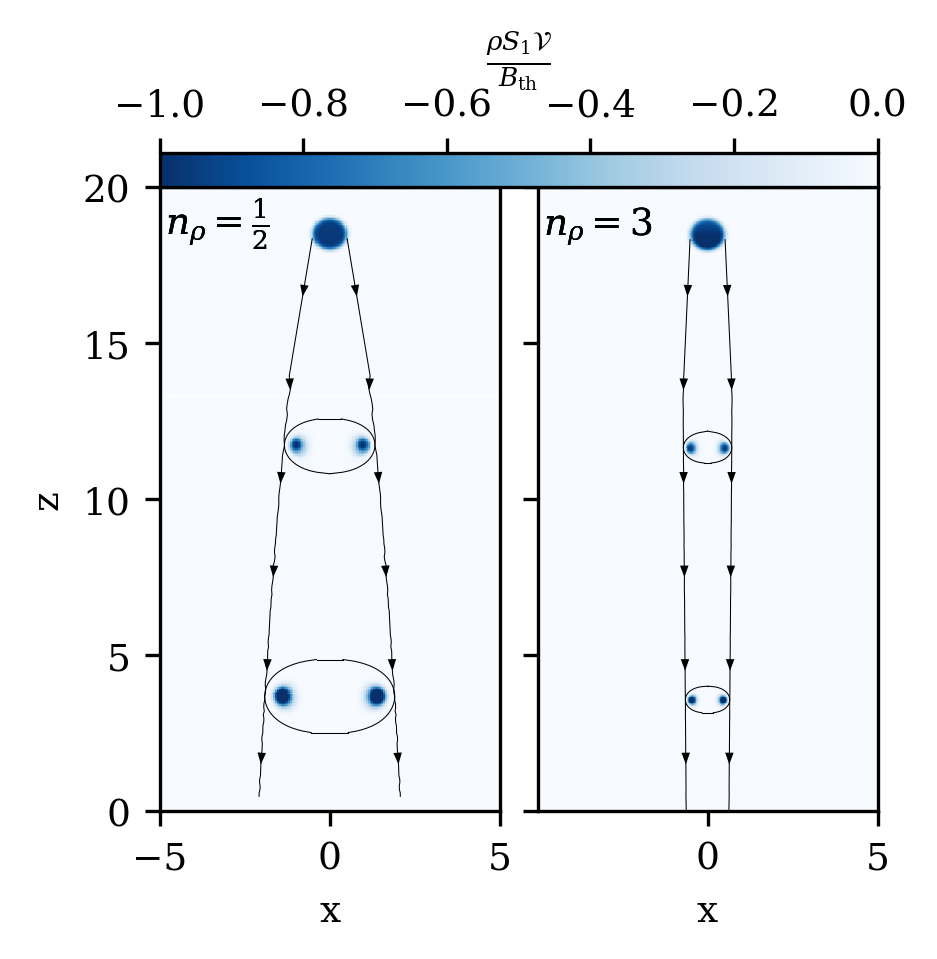
\includegraphics[width=\columnwidth]{evolution_colormeshes.png}
    \caption{
	The evolution of $\rho S_1 r^3$, the mass-weighted entropy scaled by the thermal volume, is shown for two thermals. 
	On the left is a thermal in a weakly stratified domain with $n_\rho = 1/2$ density scale heights and on the right is a thermal in a strongly stratified domain with $n_\rho = 3$.
	While both start with precisely the same initial condition, the case with low stratification expands with depth like the boussinesq case, whereas the strongly stratified thermal compresses with depth.
    \label{fig:evolution_colormeshes} }
\end{figure}


\subsection{Evolution of momentum and impulse}
The evolution of thermals as buoyant vortex rings has been well described in the unstratified, Boussinesq limit for decades (see e.g. \LJ\,for a description and references).
While many descriptions of vortex rings assume that they evolve in a self-similar state, we will lay out a description of the momentum and impulse of the thermal and show how these quantities control the evolution of the vortex ring.

We study a fluid characterized by an ideal gas equation of state and focus on the ideal, low Mach number regime in an adiabatically stratified atmosphere. 
In this regime, a linearized equation of state describes the thermodynamics well, and the fully compressible Euler momentum equation takes the form \citep{brown&all2012},
\begin{equation}
\frac{\partial \bm{u}}{\partial t} + \bm{u}\cdot\grad\bm{u} = 
-\grad\varpi - \frac{S_1}{c_P}\bm{g},
\label{eqn:euler_momentum}
\end{equation}
where $\bm{u}$ is the velocity, $\varpi = P_1 / \rho_0$ is the reduced pressure, $S = c_V\ln T - R\ln\rho$ is the specific entropy, and thermodynamics are broken down into background (subscript 0) and fluctuating (subscript 1) components.
In this limit where the linearized equation of state is valid, $S_1 \approx c_V T_1/T_0 - R \rho_1/\rho_0$.
In this work we find it instructive to examine the full momentum, and so multiplying this equation by the full density, we obtain,
\begin{equation}
\frac{\partial (\rho\bm{u})}{\partial t} + \bm{u}\cdot\grad(\rho\bm{u}) + \rho\bm{u}(\DivU)
= -\rho\grad\varpi - \rho\frac{S_1}{c_P}\bm{g}.
\label{eqn:rho_euler_momentum}
\end{equation}
Hereafter we will define the total derivative, $D/Dt \equiv \partial/\partial t + \bm{u}\cdot\grad$, and we acknowledge that the Langrangian derivative commutes with a volume integral according to 
\begin{equation*}
\frac{d}{dt}\int_{\mathcal{V}} f dV = \int_{\mathcal{V}} \left[\frac{Df}{Dt} + f(\DivU)\right]dV,
\end{equation*}
for a volume, $\mathcal{V}$, which is advected with the fluid.
Volume-integrating Eqn.~\ref{eqn:rho_euler_momentum}, we thus find
\begin{equation}
\frac{d\bm{M}}{dt} = \int_{\mathcal{V}}\left(-\rho\grad\varpi - \rho\frac{S_1}{c_P}\bm{g}\right)dV,
\label{eqn:int_momentum_eqn}
\end{equation}
where the volume-integrated momentum is defined $\bm{M} \equiv \int_{\mathcal{V}}\rho\bm{u} dV$.
At this point we will make the assumption of a plane-parallel atmosphere in which the gravity is constant, $\bm{g} = -g\hat{z}$, and note that the z-component of the volume-integrated momentum evolves according to
\begin{equation}
\frac{d M_z}{dt} = \int_{\mathcal{V}}\left( -\rho\frac{\partial \varpi}{\partial z} + \rho g \frac{S_1}{c_P} \right)dV.
\label{eqn:Mz_definition}
\end{equation}
At this stage, it is useful to define the total buoyancy,
\begin{equation}
B \equiv \int_{\mathcal{V}} \rho\, S_1\, \frac{g}{c_P}\, dV,
\label{eqn:tot_buoyancy}
\end{equation}
as in the absence of viscosity and detrainment, this is a conserved quantity during thermal evolution (see e.g., Fig.~\ref{fig:constants}a). 
Furthermore, in the Boussinesq limit, the work of \citet{tarshish&all2018} shows that pressure terms reduce the efficacy of the buoyancy in changing the momentum by effectively reducing the buoyant acceleration by some factor $\beta \sim 0.5$. 
As a result, we approximate the growth of a thermal's vertical momentum according to
\begin{equation}
\frac{d M_z}{dt} \approx \beta B.
\label{eqn:theory_momentum}
\end{equation}

We now turn our attention to the hydrodynamic impulse, which in the stratified limit can be expressed as \citep{shivamoggi2010},
\begin{equation}
\bm{I} = \frac{1}{2}\int_{\mathcal{V}} \bm{x}\times(\grad\times(\rho\bm{u}))dV,
\end{equation}
where $\bm{x}$ is the position vector. 
The hydrodynamic impulse is the time-integrated work which has acted on the fluid to result in the current fluid motion. 
Per \citet{shivamoggi2010}, changes in the impulse can be expressed as
\begin{equation*}
\frac{d\bm{I}}{d t} = \int_{\mathcal{V}}\frac{\partial(\rho\bm{u})}{\partial t}dV
= B\hat{z} - \int_{\mathcal{V}}\left[\rho\grad\varpi + \Div{\rho\bm{u}\bm{u}}\right]dV ,
\end{equation*}
where, importantly, the \emph{eulerian} time derivative of the momentum is inside of the volume integral here. 
Under the proper specification of volumetric boundaries, the integral term is zero, and the vertical impulse of a thermal thus straightforwardly changes in time as
\begin{equation}
\frac{d I_z}{d t} = B.
\label{eqn:change_in_impulse}
\end{equation}
We have thus retrieved the two findings on which our theory of thermal evolution will be built: \emph{both the impulse and momentum experience constant changes in time determined by the buoyant nature of the thermal}.

In the low-Mach number limit in which changes in density from the background are negligible, and in the limit of a thin-core vortex ring, the impulse of a vortex ring can be approximated as
\begin{equation}
I_z \approx \pi \rho r^2 \Gamma,
\label{eqn:impulse_approx}
\end{equation}
where $r$ is the radius of the thermal from its axis of symmetry to the maxima of its buoyant signature, and $\Gamma = \int_{\mathcal{A}} (\grad\times\bm{u})dA$ is the circulation in a cross-section of the vortex ring.
Integrating the momentum equation in the absence of viscous effects shows that changes in circulation in an axisymmetric vortex ring are
\begin{equation}
\frac{d\Gamma}{dt} = \oint_{\mathcal{C}} g \frac{S_1}{c_P}\hat{z} \cdot d\bm{x},
\label{eqn:circulation}
\end{equation}
where $\mathcal{C}$ is the contour around the area $\mathcal{A}$ in which the circulation is contained and $d\bm{x}$ is the line integral element around that contour.
For the case of a vortex core in which the entropic signature is contained tightly in the core, as in Fig.~\ref{fig:evolution_colormeshes}, any contour which is drawn around the vortex core should conserve circulation in the absence of viscosity.
As a result, we will treat the circulation of a developed vortex ring as a conserved quantity.


\subsection{Parameterized description of thermal evolution}
\begin{figure}[t!]
    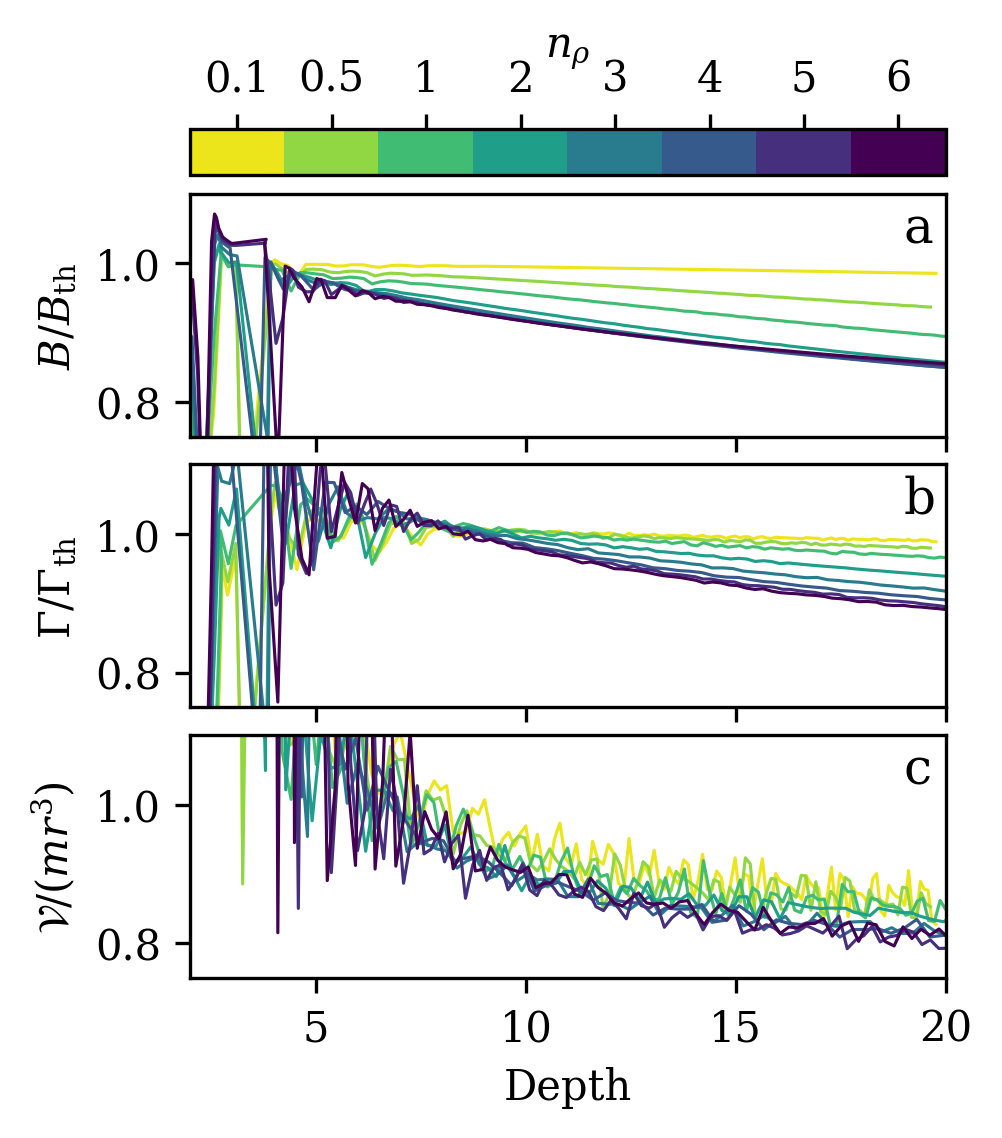
\includegraphics[width=\columnwidth]{constants.png}
    \caption{
	Evolution traces are shown for  three quantities which we assume to be constant in our parameterized thermal theory. 
	The circulation (a) and buoyancy (b), divided by their parameterized value for each case (see Table \ref{table:parameters}), are plotted vs. depth. 
	We see that with increasing stratification, there is marginally more detrainment of both of these quantities, but to first order they are constant over the	thermal's transit time. 
	In (c) the volumetric constant $f$ is shown; after significant noise during the development of the vortex ring, this quantity settles toward a value of O(7) throughout the thermal's transit.
    \label{fig:constants} }
\end{figure}

After spinning up, we assume that the thermal is characterized by a constant buoyant signature, $B_0$, and constant circulation, $\Gamma_0$.
While these thermals began as initial spherical perturbations, they can be modeled as having always been vortex rings which evolved from a ``virtual origin'' where the vortex ring is characterized by having a radius of zero. 
From this virtual origin, the vortex ring's momentum and impulse grow to a value of $M_0$ and $I_0$ at time $t = 0$ when the true thermal is released from rest.

We first note, as in Fig.~\ref{fig:constants}a, that the buoyancy in our thermals is not necessarily perfectly constant in time, and that effects like detrainment result in a minor reduction of the buoyant signature of our thermals. 
We thus express the buoyancy as 
\begin{equation}
B \approx \chi B_0,
\end{equation}
where $\chi$ is a constant of O(1) which represents this detrainment. 
We then integrate Eqn.~\ref{eqn:change_in_impulse} in time,
\begin{equation*}
I_z = \chi B_0 t + I_0.
\end{equation*}

Combining this result with Eqn.~\ref{eqn:impulse_approx}, we retrieve our first result,
\begin{equation}
r = \sqrt{\frac{\chi B_0 t + I_0}{\pi\rho\Gamma_0}}.
\label{eqn:r_theory}
\end{equation}
Following Eqn.~\ref{eqn:circulation}, and taking $\Gamma_0$ to be constant (which is a decent assumption in our numerical experiments, as in Fig.~\ref{fig:constants}b), we find that the radius grows with time but this growth is damped by increasing atmospheric density.
In the Boussinesq limit where $\rho \rightarrow \text{constant}$, we retrieve the $r \propto \sqrt{t}$ scaling found in the Boussinesq regime in \LJ. 
We find that the inclusion of stratification adds the additional complexity of $r \propto \rho^{-1/2}$, such that downward-propagating vortex rings (as studied here) will entrain less than boussinesq thermals, and upward-propagating rings will entrain more. 
In the absence of buoyancy ($B = 0$), this result aligns with the prediction for purely horizontal compression noted by \citet{brandenburg2016} of $r^2 \propto \rho^{-1}$.

The momentum can likewise be simply integrated,
\begin{equation*}
M_z = \beta\chi B_0 t + M_0.
\end{equation*}
For the proper choice of vertical velocity, $w_{\text{th}}$, and volume, $\mathcal{V}$, the momentum is also precisely 
\begin{equation*}
M_z = \rho \mathcal{V} w_{\text{th}}.
\end{equation*}
We approximate the volume as $\mathcal{V} = f r^3$, where $f$ is a parameter which we take to be constant. 
This assumption is perhaps not as perfect as the assumptions of constant $B_0$ or $\Gamma_0$ (see Fig.~\ref{fig:constants}c), but it is nevertheless not a bad assumption. 
Combining our approximate expressions, and using our theoretical description of $r$ (Eqn.~\ref{eqn:r_theory}), we retrieve
\begin{equation}
\rho^{-1/2} w_{\text{th}} = \left(\frac{(\pi \Gamma)^{3/2}}{f}\right)\frac{\beta\chi B_0 t + M_0}{(\chi B_0 t + I_0)^{3/2}}.
\end{equation}
Defining the thermal velocity $w_{\text{th}} \equiv dz_{\text{th}}/dt$, and making the assumption that the vortex ring is at the virtual origin at $t = 0$ so that $I_0 = M_0 = 0$, an integrable expression for the evolution of thermal position over time can be retrieved,
\begin{equation}
\frac{dz_{\text{th}}}{\rho(z_{\text{th}})^{1/2}} =
\left(\frac{\beta(\pi\Gamma)^{3/2}}{f(\chi B_0)^{1/2}}\right)\frac{dt}{t^{1/2}}
\label{eqn:dz_theory}
\end{equation}
If the atmospheric stratification in which the thermal is falling is known, this result can be integrated with the known profile of $\rho(z_{\text{th}})$ in order to find the position of the thermal as a function of time. 
We leave this result general for now, and will integrate it using the polytropic stratification used in our simulations in the next section.

\subsection{Solution for thermal evolution in a Polytrope}
In this work, we study an ideal gas whose equation of state is $P = \rho T$ and whose stratification is a perfectly adiabatic polytrope,
\begin{gather}
T_0 = 1 + (\grad_{\text{ad}})(z - L_z), \\
\rho_0 = T_0^{\,m_{\text{ad}}},
\label{eqn:polytrope}
\end{gather}
where $m_{\text{ad}} = (\gamma-1)^{-1}$, and where the adiabatic temperature gradient in our nondimensional systems (see section \ref{sec:experiment}) is $\grad_{\text{ad}} \equiv g(e^{n_\rho/m_{\text{ad}}} - 1)/(L_z c_P)$, with $g = m_{\text{ad}} + 1$ and $L_z = 20$ is the nondimensional depth of the atmosphere in units of thermal diameters.
 
Integrating Eqn.~\ref{eqn:dz_theory} under this polytropic density stratification and assuming $m_{\text{ad}} < 2$, we find
\begin{equation}
z_{\text{th}} = \grad_{\text{ad}}^{-1}\left[\left(\frac{2C}{ \alpha } \sqrt{t + t_{\text{off}}} + T_0^{1/\alpha}  \right)^{\alpha} - 1\right] + L_z,
\label{eqn:theory_z}
\end{equation}
where $C \equiv \beta \pi^{3/2} \grad_{\text{ad}} / f \sqrt{\Gamma^3/(\chi B)}$ and the temperature at the virtual origin is $T_0 = 1 + \grad_{\text{ad}}(z_0 - L_z)$.
The virtual origin is located at $z = z_0$ and $t = -t_{\text{off}}$ in simulation units, which are the height and time a which the vortex ring would have had zero radius in the absence of a spin-up phase.
The constant $\alpha^{-1} = 1 - m_{\text{ad}}/2$, and in the limit of large stratification, we find that $z_{\text{th}} \propto t^2$ for our case of $\alpha = 4$. 

The thermal is initialized as a uniform sphere of dense fluid, and it quickly spins up into a vortex ring. 
While we do not attempt to model the spin-up phase in this paper, it can be parameterized by the buoyancy $B_0$, circulation $\Gamma_0$, as well as the virtual origin $z_0$, and temporal offset $t_{\text{off}}$. 
Our theory also involves the volumetric aspect ratio of the thermal $f$, the detrainment fraction $\chi$, and the effective buoyancy $\beta$. 
These appear to be constant or only weakly dependent on the stratification for the thermals we have simulated.


%%%%%%%%%%%%%%%%%%%%%%%%%%%%%%%%%%%%%%%%%%%%%%%%%%%%%%%%%%%%%%%%%%%%%%%%%%%%%%%
%% EXPERIMENT SECTION
\section{Numerical Experiment} 
\label{sec:experiment}
%In this work, we primarily study the evolution of 2D, azimuthally symmetric, anelastic thermals in cylindrical coordinates. 
As a result of our theory being largely derived in the anelastic, axisymmetric limit, we have chosen to focus the bulk of our attention on our 2D, axisymmetric anelastic simulations.
We choose to focus on 2D simulations, as they allow us to more easily study high density stratifications using highly reproducible simulations whose computational expense is low.
We verify that select anelastic simulations produce the same results as 3D fully compressible simulations in cartesian domains. 

While natural processes are very turbulent, we have chosen to study the evolution of laminar thermals here. 
As we are not aware of a developed laminar theory in the stratified regime in the literature, like the one developed here, it is useful to restrict our study to the laminar case to determine the validity of our theory.
Furthermore, \LJ\, showed in the Boussinesq limit that the measured entrainment of turbulent thermal vortex rings is well described by laminar theory, and we have no reason to believe that result should not hold for the stratified case.
As a result, we leave studies of turbulent thermals to future work.

\subsection{Anelastic Simulations}
The LBR anelastic equations are \citep{lecoanet&all2014},
\begin{gather}
\DivU = -w \partial_z \ln\rho_0, \\
\begin{split}
\partial_t \bm{u} + \bm{u}\cdot\grad&\bm{u} = \\
- \grad \varpi + S_1\hat{z} &
+ \frac{1}{\rho_0\text{Re}}\left[\grad^2 \bm{u} + \frac{1}{3}\grad(\DivU)\right] 
\end{split}\\
\begin{split}
\partial_t S_1 + \bm{u}\cdot\grad S_1 =& \\
\frac{1}{\text{Re}}\left(\frac{1}{\text{Pr}\rho_0c_P }\right.&[\grad^2 S_1 + \partial_z\ln T_0 \cdot\partial_z S_1]\\
&+ \left.\frac{-(\grad_{\text{ad}})}{\rho_0 T_0}\sigma_{ij}\partial_{x_i}u_j \right),
\end{split}
\end{gather}
where $\lilstressT$ is the viscous stress tensor in units of inverse time.
In our azimuthally symetric domain, we assume that $\partial_\phi = 0$; as the initial conditions of our simulations are at rest and have no azimuthal velocity, $u_\phi$, we explicitly impose that $u_\phi = 0$; therefore $\bm{u} = u_r \hat{r} + w\hat{z}$. 

These equations have been nondimensionalized in the same manner as in \citet{lecoanet&jeevanjee2018} such that the length scale is the diameter of the initial thermal perturbation and the velocity scale is the freefall velocity. 
The timescale is thus the freefall crossing time of this unit length. 
These equations are then fully specified in terms of the Reynolds number and Prandtl number,
\begin{equation}
\text{Re} = \frac{ u_{\text{th}} L_{\text{th}}}{\nu}, \qquad
\text{Pr} = \frac{ u_{\text{th}} L_{\text{th}}}{\chi}, \qquad
u_{\text{th}}^2 = \frac{g L_{\text{th}} \Delta s}{c_P},
\end{equation}
where $u_{\text{th}}$ is the freefall velocity, $L_{th}$ is the thermal length scale, and
$\Delta s$ is the magnitude of the specific entropy signature of the thermal.

We choose an atmospheric model in which the dynamic viscosity, $\mu = \rho_0 \nu$, and the thermal conductivity, $\kappa = \rho_0 \chi$, are both uniform and constant in time.
The diffusivities $\nu$ and $\chi$ therefore scale inversely with the density.
As the diffusivities scale with depth, Re is specified at the thermal's initial depth.
All simulations conducted in this work use a value of Re = 600 and $\mbox{\text{Pr} = 1}$.

\subsection{Initial conditions}
To initialize the simulation, we specify a spherical initial specific entropy perturbation,
\begin{equation}
S_1 = - \frac{1}{2}\left[1 - \text{erf}\left(\frac{r' - r_{\text{th}}}{\delta}\right)\right].
\label{eqn:thermal_IC}
\end{equation}
Here, $r' = \sqrt{r^2 + (z - z_0)^2}$, where $z_0 = L_z - 3r_{\text{th}}$, with the thermal radius set as $r_{\text{th}} = 0.5$, and a smoothing width, $\delta = 0.1$.
As mentioned previously, Re = 600 and Pr = 1 are specified at the thermal's initial depth, $z = z_0$.

\subsection{Fully Compressible Simulations}
In order to verify the validity of our 2D Anelastic simulations, we evolve select thermals according to the 3D Navier Stokes equations in a cartesian domain. 
We use the $(T, \ln\rho)$ formulation of the equations in which we have previously studied fully compressible convection at low and high Mach number \citep{lecoanet&all2014, anders&brown2017},
\begin{gather}
\frac{\partial \ln\rho_1}{\partial t} + \epsilon^{-1}\left(\bm{u}\cdot\grad\ln\rho_0 + \DivU\right) = -\bm{u}\cdot\grad\ln\rho_1, \\
\begin{split}
\frac{\partial \bm{u}}{\partial t}  +\grad T_1 + T_1\grad\ln\rho_0 + T_0\grad\ln\rho_1  =\\
- \epsilon T_1\grad\ln\rho_1 + \frac{1}{\rho\text{Re}}\left[\grad^2\bm{u} + \frac{1}{3}\grad(\DivU)\right]
\end{split} \\
\begin{split}
\frac{\partial T_1}{\partial t} + \epsilon^{-1}\left[\bm{u}\cdot\grad T_0 + (\gamma-1)T_0\DivU\right] = \\
-\left[\bm{u}\cdot\grad T_1 + (\gamma-1)T_1\DivU\right] + \frac{1}{\rho c_V\text{Re}}\left[\frac{1}{\text{Pr}}\grad^2 T_1 + \sigma_{ij}\partial_{x_i}u_j\right].
\end{split}
\end{gather}
These equations have been nondimensionalized on the same length and timescales as the anelastic equations, use the same atmospheric profiles and assumptions, and we have explicitly assumed that the background atmosphere ($T_0, \ln\rho_0$) is in hydrostatic and thermal equilibrium in the writing of these equations. 
The new parameter $\epsilon = u_{th}^2$ is the magnitude of entropy perturbations and sets the Mach number of the thermal flows, and we use $\epsilon = 10^{-4}$ in this work. 

In setting the specific entropy to an equivalent condition to that specified in Eqn.~\ref{eqn:thermal_IC}, we note that it is essential that the initial perturbation be in pressure equilibrium. 
The set of initial conditions that achieves this is
\begin{equation}
\ln\rho_1 = S_1/c_P, \qquad T_1 = T_0(e^{-\epsilon\ln\rho_1} - 1)/\epsilon.
\end{equation}

\subsection{Numerics}
We evolve our simulations forward in time using the  Dedalus\footnote{\url{http://dedalus-project.org/}} pseudospectral framework \citep{burns&all2016} [CITE THE METHODS PAPER]. 
For our 2D simulations, we use using an implicit-explicit (IMEX), third-order, four-stage Runge-Kutta timestepping scheme RK443 \citep{ascher&all1997}, and for our 3D simulations we use the second-order semi-implicit backward differentiation formulation SBDF2 \citep{wang&ruuth2008}.

Our 3D simulations are decomposed on Fourier bases in the horizontal directions ($x, y \in [-L_r, L_r]$) and Chebyshev bases vertically ($z \in [0, L_z]$) with impenetrable, stress free, fixed-temperature boundary conditions at the upper and lower boundaries ($T_1 = w = \partial_z u = \partial_z v = 0$ at $z = [0, L_z]$).
Our 2D simulations are decomposed on a Fourier $(z \in [0, L_z])$ and Chebyshev $(r \in [0, L_r])$ domain, with boundary conditions of $\partial_r S_1 = w = (\grad\times\bm{u})_\phi = 0$ at $r = L_r$.

All of the code used to perform the simulations in this work can be found online in the supplementary materials in a Zenodo repository (CREATE AND CITE REPO).


%%%%%%%%%%%%%%%%%%%%%%%%%%%%%%%%%%%%%%%%%%%%%%%%%%%%%%%%%%%%%%%%%%%%%%%%%%%%%%%
%% RESULTS SECTION
\section{Results}
\label{sec:results}
The measured values of each of the parameters described in section \ref{sec:theory} for each of our simulations  \ref{sec:theory} for each of our simulations  \ref{sec:theory} for each of our simulations are presented in table \ref{table:parameters}.
As anticipated, $\beta$ is O(0.5) and $\chi$ is O(1), with both decreasing slightly in value with increasing stratification, which is perhaps unsurprising in light of Fig.~\ref{fig:constants}.
In all cases, the buoyancy $B_0$ is similar to the integrated buoyancy in the initial conditions, with some losses due to detrainment in the spin-up.
In our nondimensional units, we also find that the circulation is O(-2) for each of our cases, and decreases with increasing stratification (and decreasing vortex size).

\begin{deluxetable*}{c c c c c c c c}
\tabletypesize{\footnotesize}
\caption{Simulation output parameterization
\label{table:parameters}
}
\tablehead{																																															
\colhead{$n_\rho$} & \colhead{$T_0$} & \colhead{$t_{\text{off}}$} & \colhead{$B_0$} & \colhead{$\Gamma_0$} & \colhead{$f$} & \colhead{$\chi$} & \colhead{$\beta$}	}	
\startdata																																															
\multicolumn{8}{l}{\textbf{2D Anelastic Simulations}}\\
0.1 	&  0.985	& 0.166	& -0.547 & -2.17 & 7.01	& 1.04	& 0.499	\\
0.5 	&  0.918	& 0.704	& -0.568 & -2.12 & 7.04	& 0.976	& 0.490	\\
1	 	&  0.827	& 1.09 	& -0.601 & -2.05 & 7.07	& 0.915	& 0.480	\\
2	 	&  0.677	& 1.26	& -0.712 & -1.89 & 7.08	& 0.841 & 0.456	\\
3	 	&  0.619	& 1.01	& -0.946 & -1.73 & 7.08	& 0.808	& 0.436	\\
4	 	&  0.698	& 0.622	& -1.47	 & -1.59 & 7.10	& 0.793	& 0.422	\\
5	 	&  0.963	& 0.327	& -2.70	 & -1.49 & 7.15	& 0.786	& 0.414	\\
6	 	&  1.57 	& 0.064	& -5.73	 & -1.43 & 7.16	& 0.787	& 0.408	\\
\multicolumn{8}{l}{\textbf{3D Fully Compressible Simulations}}\\    
0.5 	&  0.924	& 0.583	& -0.568 & -2.12 & 6.66	& 0.978	& 0.452	\\
1	 	&  0.832	& 1.26	& -0.601 & -2.05 & 6.88	& 0.902	& 0.454	\\
2	 	&  0.666	& 1.53	& -0.711 & -1.89 & 7.08	& 0.822	& 0.450	\\
\enddata																																															
\tablecomments{ }
\end{deluxetable*}

\begin{figure}[t!]
    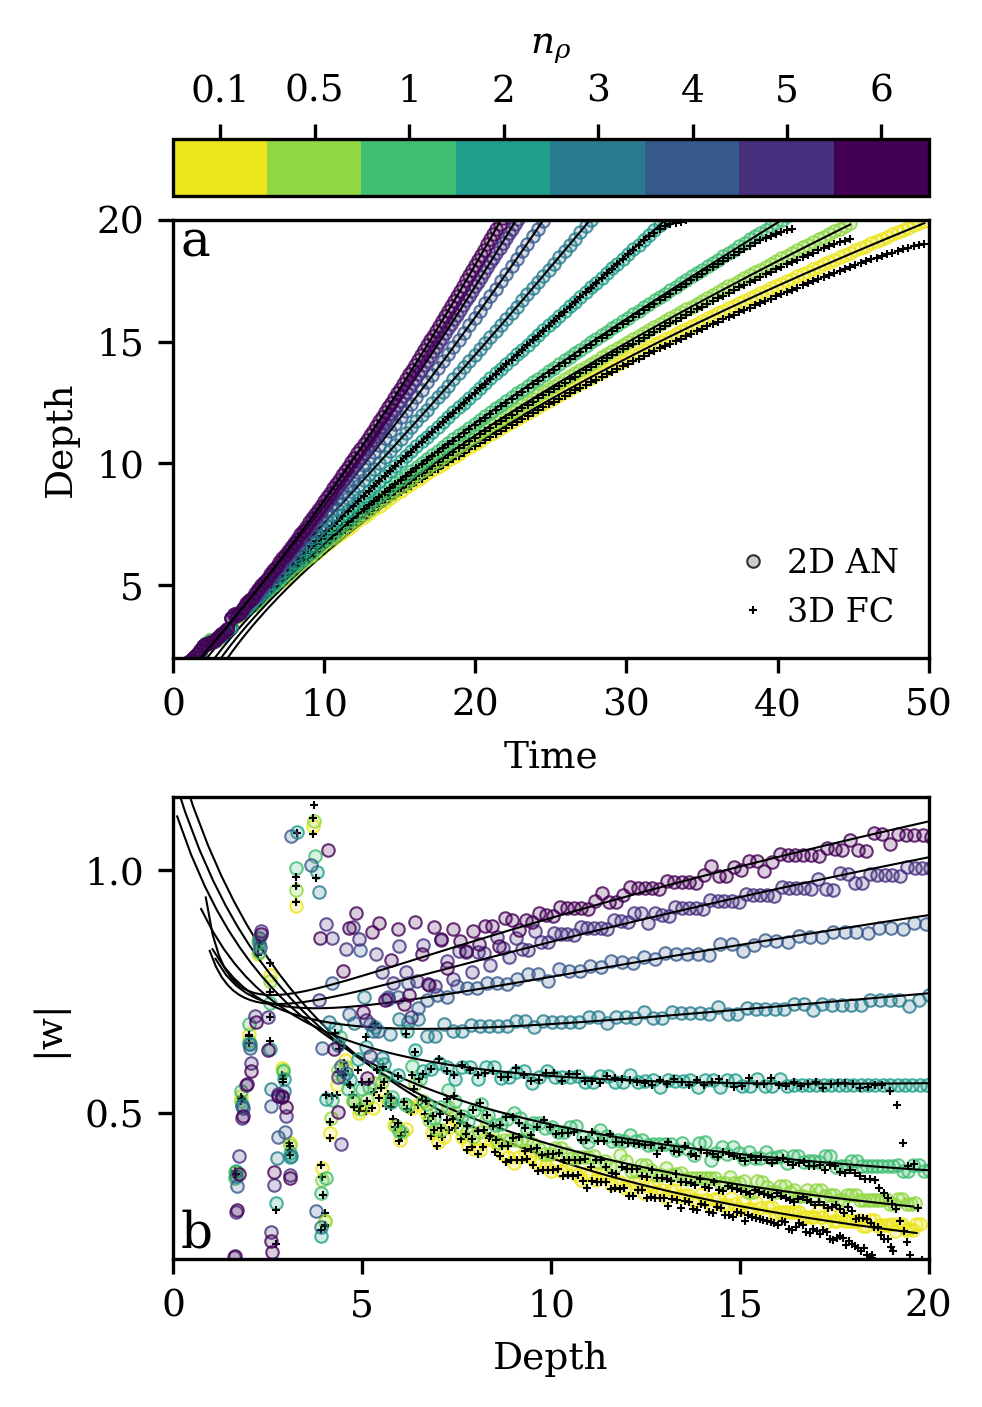
\includegraphics[width=\columnwidth]{results_panels.png}
    \caption{
	The measured depths of thermals as a function of time for all 2D Anelastic and 3D Fully compressible simulations conducted in this work are shown in (a).
	The corresponding thermal velocities as a function of depth are shown in (b)
	Overplotted in a thin solid line for each case are our theoretical predictions from section \ref{sec:theory} given the parameters in table \ref{table:parameters}.
    \label{fig:results_panels} }
\end{figure}

\begin{figure}[t!]
    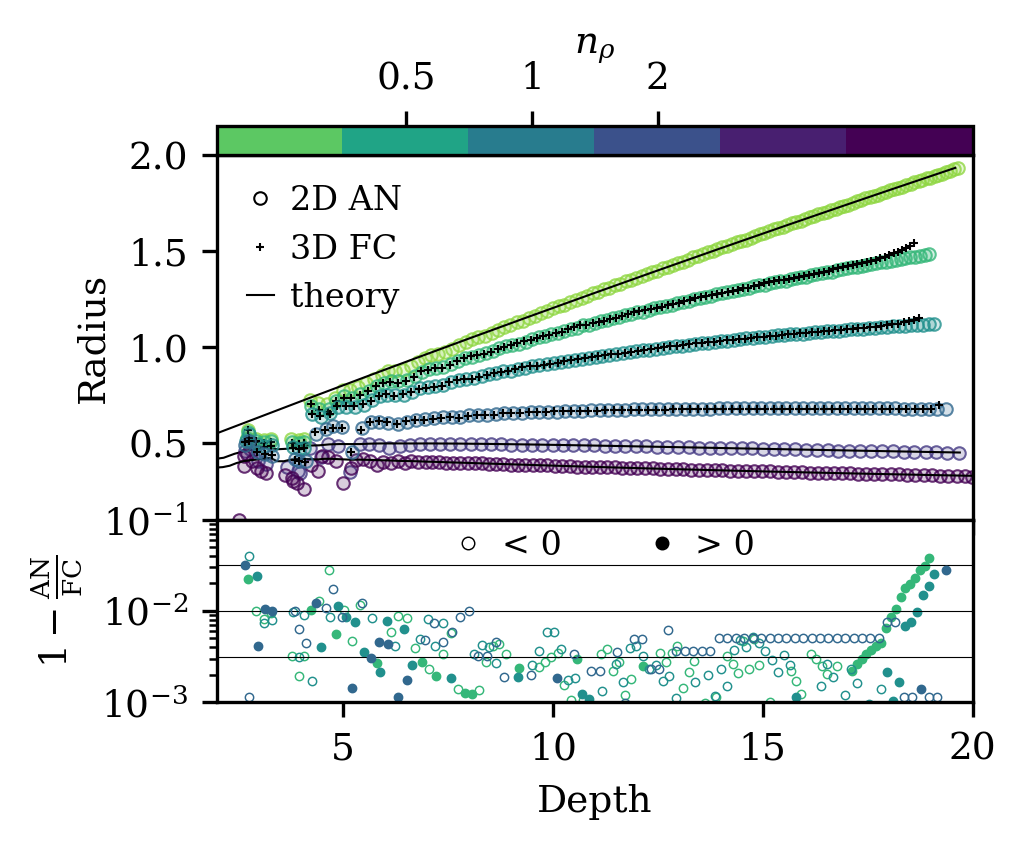
\includegraphics[width=\columnwidth]{diff_AN_FC.png}
    \caption{
	Measured values of radius vs. depth are plotted for both the 2D anelastic and 3D fully compressible simulations in (a). 
	For completeness, we also include the cases in which we only studied the 2D anelastic simulations.
	For the cases in which only the anelastic equations were solved, the theory is overplotted in a thin solid line, and similar agreement between simulations and theory is found for the cases where both equations sets were used.
	The fractional difference between anelastic and fully compressible results are shown in (b).
    \label{fig:diff} }
\end{figure}



In Fig. \ref{fig:results_panels}a, we show the measured depth $d_{\text{th}} = L_z - z_{\text{th}}$ of the thermal as a function of time for low and high stratification. 
At very low stratification (e.g., $n_\rho = 0.1$), the thermal is small compared to the local density scale height at all depths, and it evolves roughly according to the Boussinesq prediction of $d \propto \sqrt{t}$. 
As the stratification increases, the thermal begins to transit the domain more quickly and approaches the limit of $d \propto t^2$ predicted in the highly stratified limit of Eqn.~\ref{eqn:theory_z}. 
The theoretical fits for depth from the prediction of Eqn.~\ref{eqn:theory_z} are plotted over the measured data and show remarkable agreement.

In Fig.~\ref{fig:results_panels}b, we show the corresponding thermal velocity as a function of depth with the theory overplotted again.
As anticipated, low density ($n_\rho = 0.1$) thermals deccelerate with depth.
We find that with increasing stratification, this decceleration stops and sufficiently stratified runs ($n_\rho \geq 3$) experience acceleration of the thermal.

In Fig.~\ref{fig:diff}a, we display measured thermal radius vs. depth, with a detailed comparison of our 2D Anelastic and 3D Fully Compressible cases. 
In the low stratification limit, the radius of the thermal grows linearly with depth, $r \propto d$, aligning with the Boussinesq limit shown in \citet{lecoanet&jeevanjee2018}.
This growth of the thermal is the result of entrainment of environmental fluid and accompanies decceleration like $w \propto d^{-1}$ in the Boussinesq limit, as is shown in Fig.~\ref{fig:results_panels}b.
However, as stratification increases, the thermal entrainment of environmental fluid decreases and it experiences less expansion.
In the limit of large stratification ($n_\rho \geq 3$), thermals begin contracting with depth.
This lessened entrainment is, unsurprisingly, accompanied by greater acceleration of the thermal (Fig.~\ref{fig:results_panels}).


In Fig.~\ref{fig:diff}b, the fractional difference in radius vs. depth between 3D FC and 2D AN cases is shown for the $n_\rho = [0.5, 1, 2]$ cases studied here. 
Aside from early in the simulation, when the thermal is spinning up, and late in the simulation, when the 3D simulations begin interacting with the impenetrable boundary at the bottom of the domain, the 2D anelastic and 3D fully compressible simulations agree surprisingly well.
We find differences in the radius of less than 1\% throughout the bulk of the thermal evolution for the cases studied here.
This gives us confidence that our high stratification anelastic simulations are producing reliable results.
Furthermore, this close agreement between low Mach number Fully Compressible simulations and Anelastic simulations parallels the agreement between the equation sets seen in \citet{lecoanet&all2014}.

For details on how measurements of thermal properties are conducted in our simulations, we refer the reader to appendix \ref{appendix:measurements}.

%%%%%%%%%%%%%%%%%%%%%%%%%%%%%%%%%%%%%%%%%%%%%%%%%%%%%%%%%%%%%%%%%%%%%%%%%%%%%%%
%% CONCLUSION SECTION
\section{Conclusion \& Discussion}
\label{sec:discussion}
In this paper we developed a simple theory of the evolution of buoyant (or dense) vortex rings in stratified atmospheres.
We showed that this theory predicts that dense thermals will experience less entrainment than boussinesq thermals due to increasing atmospheric density with depth.
We performed 2D anelastic simulations of thermal evolution for varying degrees of stratification and showed that our parameterized theory describes the evolution of thermals in these systems remarkably well.
Furthermore, we verified the validity of our anelastic simulations with select 3D fully compressible simulations of thermal evolution and found agreement to under 1\%.

We note that the evolution of dense thermals in stratified domains is complex, and neither the assumption of horizontal compression \citep[as in e.g.][]{brandenburg2016} or the evolution of thermals in the Boussinesq regime (as in \LJ) fully describes the behavior of these events fully.
Rather, results fall somewhere in between, and theory and simulations suggest that there are two regimes of downflowing thermal behavior:
\begin{enumerate}
\item A low-stratification ``stalling'' regime, in which the thermal entrains environmental fluid and slows down, acting much like the Boussinesq regime, and
\item A high-stratification ``falling'' regime, in which the thermal falls fast enough that compression due to the atmospheric stratification results in minimal entrainment and the thermal accelerates as it falls deeper into the atmosphere.
\end{enumerate}

However, we note that both the falling and stalling regimes observed here could result in interesting problems for the entropy rain hypothesis. 
If solar convection were comprised of thermals in the stalling regime, it is unlikely that such elements would ever make it to the base of the solar convection zone.
Rather, we expect that they would stall closer to the solar surface and deposit their entropy signature there. 
This could be seen as agreeing with the hypothesis of supergranulation as the largest buoyantly driven scale of solar motion.

On the other hand, if solar convection is comprised of thermals in the falling regime, then it is not out of the question for solar surface elements to reach deep into the Sun.
While vortex rings in the falling regime would theoretically be able to reach the bottom of the solar convection zone, the compression effects that occur as they shrink could cause problems.
For example, it is possible that these thermals could shrink to the point where conductivity becomes important, or as their length scales decrease and velocities increase, viscous heating could become an important effect and essentially erase the buoyant signature of these entropy rain droplets.

In Fig.~\ref{fig:discussion}, we extrapolate the results of our simulations to solar convection.
For each simulation performed, we show the behavior of our thermals if they were to fall the first $n_\rho = 10$ density scale heights of the solar convection zone, rather than the few that we were able to simulate here.
We see blahblahblah.


\begin{acknowledgements}
This work was supported by NASA Headquarters under the NASA Earth and Space Science Fellowship Program -- Grant 80NSSC18K1199.
This work was additionally supported by  NASA LWS grant number NNX16AC92G.  
Computations were conducted with support by the NASA High End Computing (HEC) Program through the NASA  Advanced Supercomputing (NAS) Division at Ames Research Center on Pleiades with allocation GID s1647.
\end{acknowledgements}

\appendix
\section{Thermal Measurements}
\label{appendix:measurements}
Throughout this work, we frequently report the thermal's radius or its depth.
We measure the thermal's radius and height as the radius from the axis of symmetry and the height from the bottom of the domain at which the thermal's vortex core is located.
To measure this, we locate the maxima of the entropy.
To find the entropy maxima vertically, we integrate $\int\rho S_1 r dr$ in our Dedalus domain, then use the spectral data of that profile to sample it on a 4096 point grid vertically, and we take the location of the minima on that grid to be the thermal height.
To find the entropy maxima horizontally, we integrate $int \rho S_1 dz$ in our Dedalus domain, then sample the spectral data onto a 2048-point radial grid, and take the minima of that profile to be the radius of the thermal.
In order to find the thermal's velocity as a function of time, we use a five-point stencil to differentiate the thermal's depth, $d$,
$$
w_{\text{th}}(t) = \frac{d }{dt}d_{\text{th}}(t) = \frac{-d_{\text{th}}(x + 2\Delta t) + 8d_{\text{th}}(t + \Delta t) - 8 d_{\text{th}}(t - \Delta t) + d_{\text{th}}(t - 2\Delta t)}{12\Delta t}
$$

Integral quantities, such as the circulation, $\Gamma$, the buoyancy, $B$, and the volume, $\mathcal{V}$ require us to first determine what fraction of the domain constitutes the thermal.
To do so, we use the thermal tracking algorithm described in appendix \ref{appendix:tracking} to determine the radial contour that outlines the thermal as a function of height, $\mathcal{C}$.
We then use this contour to find our integral quantities,
\begin{equation}
\Gamma = \int_0^{\mathcal{C}}\int_0^{L_z} (\grad\times\bm{u})_\phi dz dr, \qquad
B      = \int_0^{\mathcal{C}}\int_0^{L_z} \rho S_1 dz dr, \qquad
\mathcal{V} = \int_0^{\mathcal{C}}\int_0^{L_z} 1\,dz dr.
\end{equation}

\section{Thermal Tracking}
\label{appendix:tracking}
We use a thermal tracking algorithm very similar to the one used in  \citet{lecoanet&jeevanjee2018} and inspired by the work of \citet{romps&all2015} in order to determine the full extent of the thermal, as pictured by the elliptical outlines in Fig.~\ref{fig:evolution_colormeshes} 
We begin by measuring the thermal's velocity versus time, $w_{\text{th}}$, as described in appendix \ref{appendix:measurements}. 
We then calculate the streamfunction of the velocity field as in \citet{romps&all2015},
\begin{equation}
\frac{\partial \psi}{\partial r} = 2\pi \rho r (w - w_{\text{th}}),
\end{equation}
with the boundary condition that $\psi = 0$ at $r = 0$. 
The contour defined by $\psi = 0$ from this solution is taken to be the contour bounding the thermal, $\mathcal{C}$.


\section{Table of Simulations}
\label{appendix:table}
Information regarding the simulation resolution and CFL safety factor for each of the simulations presented in this work is contained in table \ref{table:simulation_info}.
The Python scripts used to perform all simulations and analysis in this work are stored online in a Zenodo repository CITE.

\begin{deluxetable*}{c c c c c c}
\tabletypesize{\footnotesize}
\caption{Table of simulation information
\label{table:simulation_info}
}
\tablehead{																																															
\colhead{$n_\rho$} & \colhead{$L_r$} & \colhead{nr or nx = ny} & \colhead{nz} & \colhead{$t_{\text{evolution}}$} & \colhead{safety}	}	
\startdata																																															
\multicolumn{6}{l}{\textbf{2D Anelastic Simulations}}\\
0.1 	& 	5				&	128			& 512			& 50 	&	0.6	\\
0.5 	& 	5				&	128			& 512			& 45 	&	0.6	\\
1	 	& 	5				&	128			& 512			& 41 	&	0.6	\\
2	 	& 	5				&	256			& 1024			& 34	&	0.4	\\
3	 	& 	5				&	256			& 1024			& 29	&	0.4	\\
4	 	& 	5				&	256			& 1024			& 26 	&	0.3	\\
5	 	& 	5				&	256			& 1536			& 25 	&	0.14	\\
6	 	& 	5				&	256			& 1536			& 23 	&	0.08	\\
\multicolumn{6}{l}{\textbf{3D Fully Compressible Simulations}}\\
0.5 	& 	5				&	256			& 512			& 42.5 		&	0.2	\\
1	 	& 	4				&	256			& 512			& 38 	 	&	0.2	\\
2	 	& 	3.5				&	256			& 1536			& 31.75 	&	0.2	\\
\enddata																																															
\tablecomments{
}
\end{deluxetable*}

\bibliography{../tex/biblio.bib}

\listofchanges
\end{document}
